\documentclass[titlepage, a4paper, 11pt, dvipdfmx]{jsarticle}
\usepackage{customstyle}

\title{\Huge【レポート\#1】ラグランジュ補間}%タイトル
\date{\today}%日付
\author{\Large BV20036 \quad 大野 弘貴}%名前

\begin{document}
\maketitle
\pagenumbering{roman}
% \tableofcontents%目次が消したい場合はコメントアウト
\newpage
\pagenumbering{arabic}

%%%%%%%%%%%%%%%%%%%%%%%%%%%%%%%%%%%%%%%%%%%%%%%%%%%%%%%%%%%%%%%%%%%%%%%%%%%%%
%%%%%%%%%%%%%%%%%%%%%%%%%%%%%%%%%%%%%%%%%%%%%%%%%%%%%%%%%%%%%%%%%%%%%%%%%%%%%
%%%%%%%%%%%%%%%%%%%%%%%%%%%%%%%%%%%%%%%%%%%%%%%%%%%%%%%%%%%%%%%%%%%%%%%%%%%%%
%以下サンプル%ここから書き始めてください

%セクション(目次に表示されるのは初期設定では)
\section{レポート内容}
\begin{itembox}[l]{囲いのタイトル左版}
    \begin{itemize}
        \item 標本点が次の (真の) 関数により与えられる場合を考える\\
      $$ f(x)=\frac{1}{1+2x^2} $$
        \item n+1個の標本点($x_0$,$f_0$), ($x_1$,$f_1$), $ \cdots $, ($x_n$,$f_n$)が区間[-5, 5]において等間隔で与えられていたとする
        \begin{itemize}
            \item 上記の真値となる関数から自分で(自動で)標本点を作成する
        \end{itemize} 
        \item 区間[-5, 5]を100等分したときの分点101点ラグランジュ補間を計算し、グラフを作成せよ
        \item n = 5, 8, 11, 14について真値の関数, ラグランジュ補完を計算し, グラフを作成せよ
        \begin{itemize}
            \item nは多項式の次数,標本点の数は(n+1)個
        \end{itemize} 
  \end{itemize}
    \end{itembox}
    \section{レポート内容}
\subsection{サブセクション}
\subsubsection{サブサブセクション}

%囲い
\begin{itembox}[l]{囲いのタイトル左版}
複数行の四角の囲い.
\end{itembox}

\begin{itembox}[c]{囲いのタイトル中央版}
複数行の四角の囲い. 囲いのタイトル左版
\end{itembox}

\begin{itembox}[r]{囲いのタイトル右版}
複数行の四角の囲い.
\end{itembox}

%改ページ
\newpage

%箇条書き
\begin{itemize}
\item 箇条書き
\item 箇条書き
\item 箇条書き
\end{itemize}

\begin{itemize}
\item 箇条書き
\item 箇条書き
\item 箇条書き

\begin{itemize}
\item 箇条書きの中にも箇条書きを入れられる
\item 箇条書きの中にも箇条書きを入れられる
\item 箇条書きの中にも箇条書きを入れられる

\begin{itemize}
\item 箇条書きの中にも箇条書きを入れられる
\item 箇条書きの中にも箇条書きを入れられる
\item 箇条書きの中にも箇条書きを入れられる

\begin{itemize}
\item 箇条書きの中にも箇条書きを入れられる
\item 箇条書きの中にも箇条書きを入れられる
\item 箇条書きの中にも箇条書きを入れられる
\end{itemize}

\end{itemize}

\end{itemize}

\end{itemize}

%番号付き箇条書き
\begin{enumerate}
\item 数字つき箇条書き
\item 数字つき箇条書き
\item 数字つき箇条書き
\end{enumerate}

\begin{enumerate}
\item 数字つき箇条書き
\item 数字つき箇条書き
\item 数字つき箇条書き

\begin{enumerate}
\item 数字つき箇条書き
\item 数字つき箇条書き
\item 数字つき箇条書き

\begin{enumerate}
\item 数字つき箇条書き
\item 数字つき箇条書き
\item 数字つき箇条書き

\begin{enumerate}
\item 数字つき箇条書き
\item 数字つき箇条書き
\item 数字つき箇条書き
\end{enumerate}

\end{enumerate}

\end{enumerate}

\end{enumerate}

%見出し付き箇条書き
\begin{description}
\item[あいうえお] 見出し付き箇条書き
\item[かきくけこ] 見出し付き箇条書き
\item[さしすせそ] 見出し付き箇条書き
\end{description}

%画像挿入
\begin{figure}[H]
\begin{center}%中央寄せ用
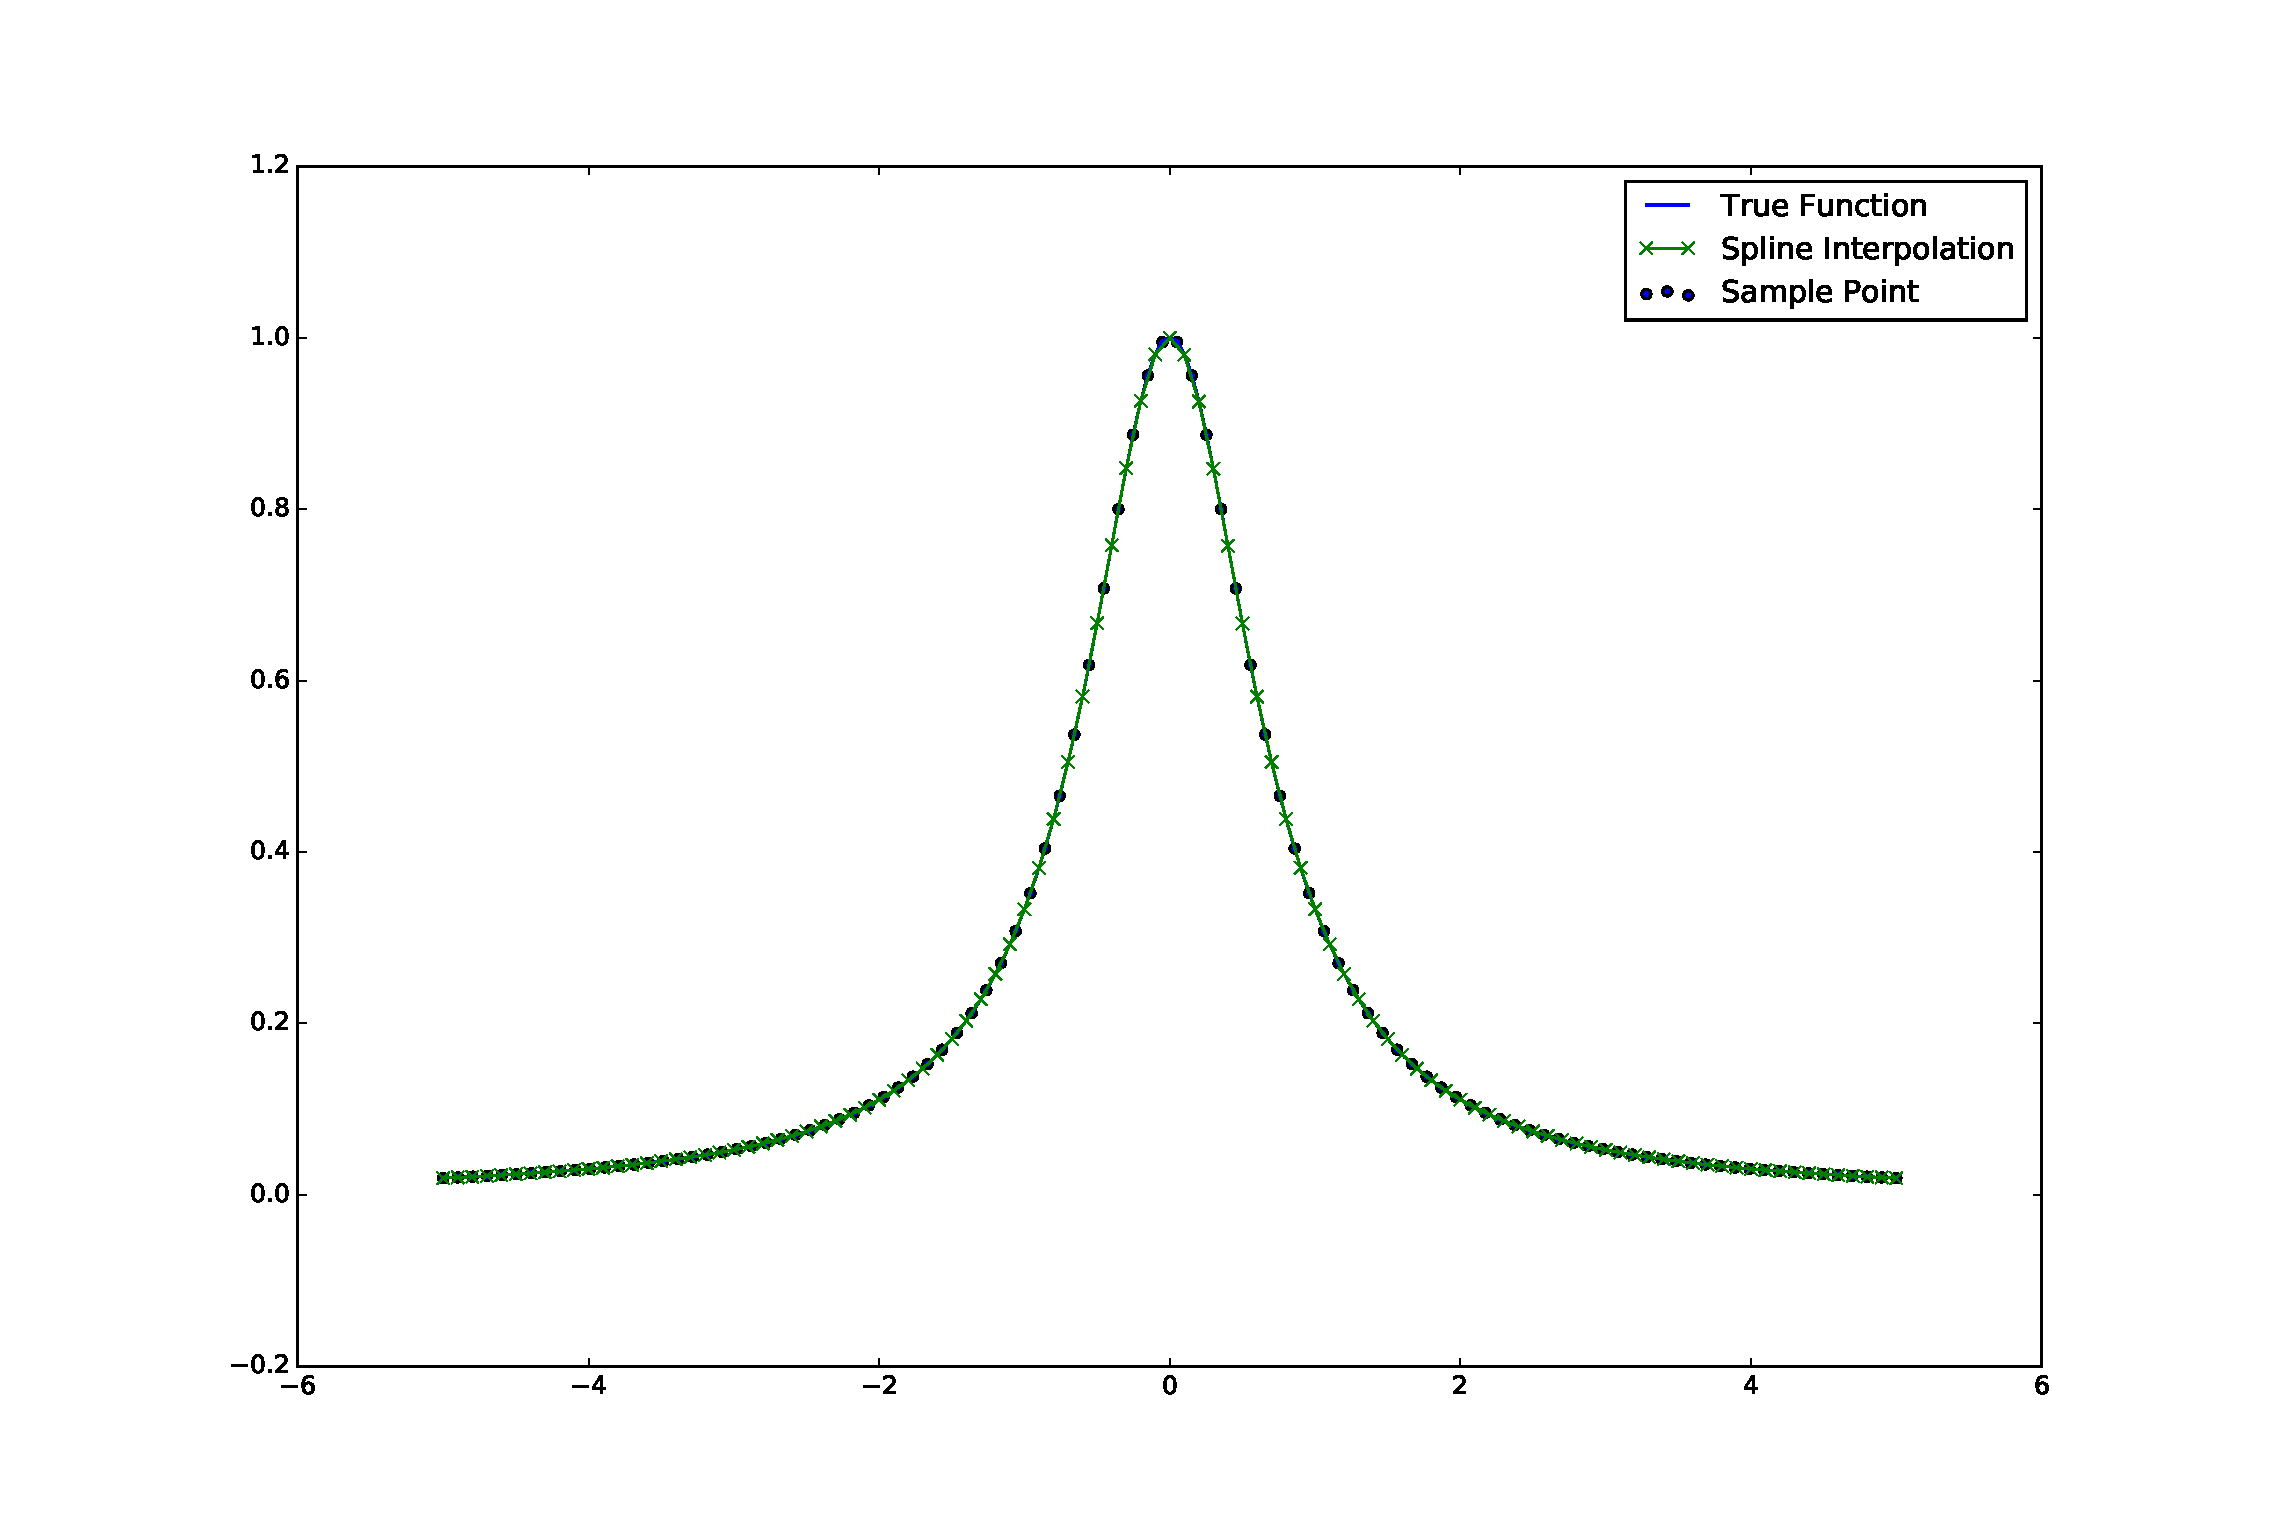
\includegraphics[width=13.5cm]{./graphics/graph.eps}%[大きさ指定]{ファイルの相対パス}
\caption{キャプション}
\label{Label}%ラベル
\end{center}
\end{figure}
%ラベルは\ref{Label}のように書くと数字だけ表示される(2回コンパイルが必要). {括弧}の中身は任意(英語推奨).

%プログラム挿入
\lstinputlisting[caption=キャプション, label=Label_Program]{./program/program.c}%[キャプションやらラベルやら]{ファイルの相対パス}

\begin{lstlisting}[caption=キャプション, label=Label_Program_2]
#include<stdio.h>
int main{
    printf("Hello World!!");
    return 0;
}
\end{lstlisting}

%参考資料記載
\begin{thebibliography}{1}
%著者, タイトル, 出版社, 現在の版の第1刷が発行された年. など, 詳しくはググる
\bibitem{kaggle} 門脇大輔 他, Kaggleで勝つデータ分析の技術 : 2019.10.22
%\bibitem{ラベル名}, \cite{ラベル名}で呼び出せる(2回コンパイルが必要)
\end{thebibliography}


\end{document}
